\clearpage
\section{Phase 5: Legal Statute Identification}
\label{sec:phase5}

\subsection{Task and experimental design}
A legal case can invoke several statutes. The input is a case identifier and
case text. The output is a nonempty set of integer statute identifiers from
\(\{0,\ldots,99\}\). We encode the gold set as
\(y\in\{0,1\}^{100}\) and model each marginal with a sigmoid. A softmax would
force the labels to compete for a single unit of probability. The official
metric is macro-F1,
\[
 F_{\mathrm{macro}}=\frac{1}{100}\sum_{j=0}^{99}
 \frac{2\,\mathrm{TP}_j}{2\,\mathrm{TP}_j+\mathrm{FP}_j+\mathrm{FN}_j}.
\]
A zero denominator contributes zero in local evaluation. Micro-F1 pools
counts before taking the ratio. Exact-set accuracy requires all labels to
agree on a case. Official scores use hidden test labels. The published
development metrics use the same labeled cases as threshold selection, so
they measure fit on the calibration set.

\subsection{Corpus and input coverage}
The pinned \path{Phase_5_LSI} revision supplies 42,750 training cases, 10,181
labeled development cases and 13,019 hidden-label test cases. The notebook
groups training documents by the SHA-256 of their exact text and uses a
10\% group holdout with seed 42. This assigns 38,444 cases to optimization
and 4,306 to checkpoint selection, with all 100 labels represented in the
internal holdout. The official splits have disjoint IDs. The notebook
counted 81 shared exact texts between official train and development and 108
between train and test. Shared text weakens the independence of the
official partitions. Its effect on results has not been isolated.

\begin{table}[htbp]
\centering\small
\caption{Official split sizes and input lengths. BPE lengths for training
refer to the 38,444 core cases. Character percentiles describe the original files.}
\label{tab:p5-corpus}
\begin{tabular}{lrrrrr}
\toprule
Split & Cases & Unique texts & Median chars & Median BPE & \(>1530\) BPE \\
\midrule
Train & 42,750 & 42,315 & 2,717 & 637 & 31.0\% \\
Development & 10,181 & 10,118 & 3,418 & 799 & 35.7\% \\
Test & 13,019 & 12,940 & 3,368 & 787 & 34.5\% \\
\bottomrule
\end{tabular}
\end{table}

Mean cardinality is 3.705 in training and 3.916 in development, with densities
of 3.70\% and 3.92\% across 100 labels. Training support varies from 272 cases
(statute 84) to 11,730 (statute 5), a factor of 43. Statutes 34 and 97 occur
in 10,380 and 7,880 training cases. Frequent development pairs include
\((5,34)\) in 912 cases, \((43,97)\) in 862 and \((12,13)\) in 849. The
shared case representation can learn correlations through its features.
The classifier has no explicit rule or structured loss for label pairs (Figure~\ref{fig:p5-labels}).

\begin{figure}[htbp]
\centering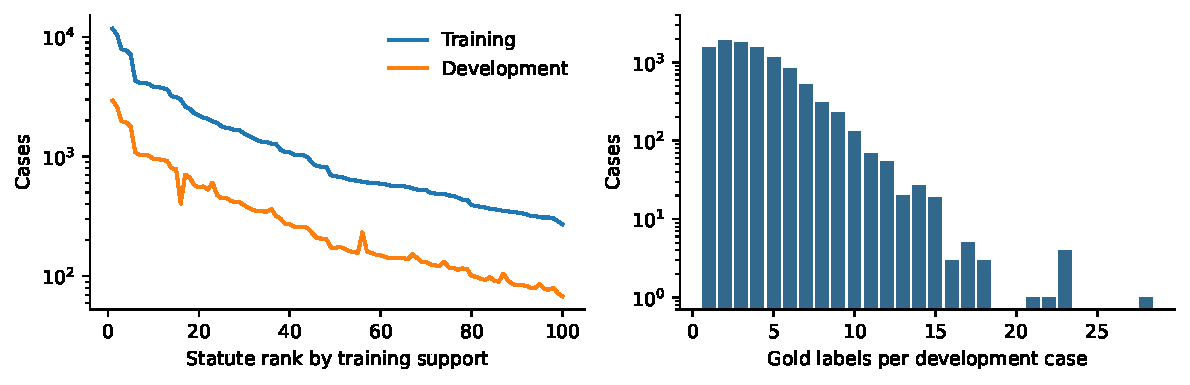
\includegraphics[width=.94\linewidth]{figures/phase5/p5_labels.pdf}
\caption{Statute support on the labeled splits and development label cardinality.}
\label{fig:p5-labels}
\end{figure}

The original legal 32k byte-level BPE uses PAD/BOS/EOS/UNK IDs 0/1/2/3.
Documents of up to 510 BPE tokens occupy one window. Longer documents use
three spans of 510 tokens with starts at the rounded equally spaced
positions from 0 to \(L-510\). BOS and EOS surround each span and each
window has capacity 512. Windows can overlap. When \(L>1530\), unsampled
tokens fall between windows. The 95th-percentile length is about 6,017
BPE tokens in the core and 6,482 in development. The average development
case retains 82.3\% of its tokens under the three-window policy, with
each case weighted equally. Evidence confined to an unsampled gap is
unavailable to the model.

\subsection{Document representation and adaptation}
For each active window \(k\), the classifier reads the EOS hidden state
\(h_k\) and applies layer normalization, dropout at 0.10 and a linear
projection \(s_k=W\,\mathrm{Dropout}(\mathrm{LN}(h_k))+b\).
Causal backbones read the EOS position after all preceding window tokens.
Prefix-LM uses the complete unpadded window as a bidirectional prefix.
Encoder--decoder uses the unpadded encoder states and leaves its
autoregressive decoder outside the classifier's forward path. The
statute-wise document logits are
\[
 z_j = \frac{\log\sum_{k=1}^{K}\exp(2s_{kj})-\log K}{2}.
\]
Here \(K\) counts active windows and the subtraction normalizes the pool
when all window scores agree. Larger window logits carry more weight, and
different windows can provide evidence for different statutes. Padding
does not contribute to the pool. The model does not exchange attention
across windows.

\begin{table}[htbp]
\centering\small
\caption{Executed configurations and best internal validation epochs.
Epoch selection used macro-F1 at a fixed threshold of 0.30.}
\label{tab:p5-models}
\begin{tabularx}{\linewidth}{ll>{\raggedright\arraybackslash}Xrrrr}
\toprule
Run & Foundation & Adaptation & Objective & LR & Epochs & Best ep. \\
\midrule
E01 & GQA 700M & Rank-8 LoRMA+ & W-BCE & \(4{\times}10^{-4}\) & 4 & 4 \\
E02 & GQA 700M & Full fine-tuning & ASL & \(2{\times}10^{-5}\) & 3 & 3 \\
E03 & Decoder 100M & Last four blocks and final norm & W-BCE & \(8{\times}10^{-5}\) & 4 & 3 \\
E04 & Prefix-LM 100M & Width-32 projection adapters & W-BCE & \(4{\times}10^{-4}\) & 4 & 4 \\
E05 & Encoder--decoder 100M & Rank-8 LoRA & ASL & \(4{\times}10^{-4}\) & 4 & 3 \\
E06 & GQA 700M & Six inherited blocks, full tuning & KD & \(4{\times}10^{-5}\) & 4 & 3 \\
\bottomrule
\end{tabularx}
\end{table}

All initial weights came from the Phase 1 official-data models.
The executed notebook recorded strict-load checks for all four foundation
snapshots. E01 freezes the GQA backbone and places low-rank corrections on
the attention projections. For a frozen projection \(u=W_0x+b_0\), the
notebook's LoRMA+ computes \(u+(16/r)BAu\). E05 uses the LoRA form
\(u+(16/r)BAx\). Both initialize \(B\) to zero. E04 wraps attention
projections with \(u+U\,\mathrm{GELU}(Du+d)+c\), initializing the up projection
and its bias to zero. E03 updates the top four decoder blocks and the final
normalization, alongside the task head. E02 trains the complete GQA
classifier. E06 retains GQA blocks 0, 3, 5, 8, 10 and 13 from the original
Phase 1 initialization and trains 62.41 million parameters, compared with
about 113 million in the full classifiers.

\subsection{Objectives, training and checkpoint selection}
Weighted binary cross-entropy multiplies the positive loss term for label
\(j\) by
\[
 w_j=\operatorname{clip}_{[1,8]}
 \sqrt{\frac{N-f_j}{\max(f_j,1)}},
\]
where \(f_j\) counts positives in the core. Asymmetric loss (ASL) uses
\[
 \ell_j=-y_j\log p_j-(1-y_j)p_j^4\log\min(1,1-p_j+0.05).
\]
The implementation clamps both logarithm inputs away from zero.
The clip and exponent downweight easy negatives. The loss averages
across labels. E06 uses
\[
 \mathcal{L}_{\mathrm{KD}}=
 \tfrac12\mathcal{L}_{\mathrm{W\text{-}BCE}}+
 \tfrac12T^2\,\mathrm{BCE}
 \bigl(\sigma(z_{\mathrm{s}}/T),\sigma(z_{\mathrm{t}}/T)\bigr),
 \qquad T=2.
\]
The soft term supervises each statute independently with cached E01
document logits. E01 scored 0.3210 on internal validation at threshold
0.30 versus E02's 0.2203, so the notebook chose E01 as teacher before
development calibration. No matched six-layer gold-only control was
archived.

The optimizer is AdamW at a fixed run-specific rate, with weight decay
0.01, one case per backward pass, accumulation over 16 cases and gradient
norm clipping at 1. The final partial group uses the same divisor.
The resume notebook carried training across two environments. It
restored model, optimizer, mixed-precision scaler when applicable, the
deterministic epoch order, the next document and the random state at
optimizer boundaries. In the executed continuation, E01--E04 reported
completed training, E05 resumed through its fourth epoch, and E06 trained
after the teacher was selected. The public port reads the same local
checkpoint state fields and saves new checkpoints atomically.

\begin{figure}[htbp]
\centering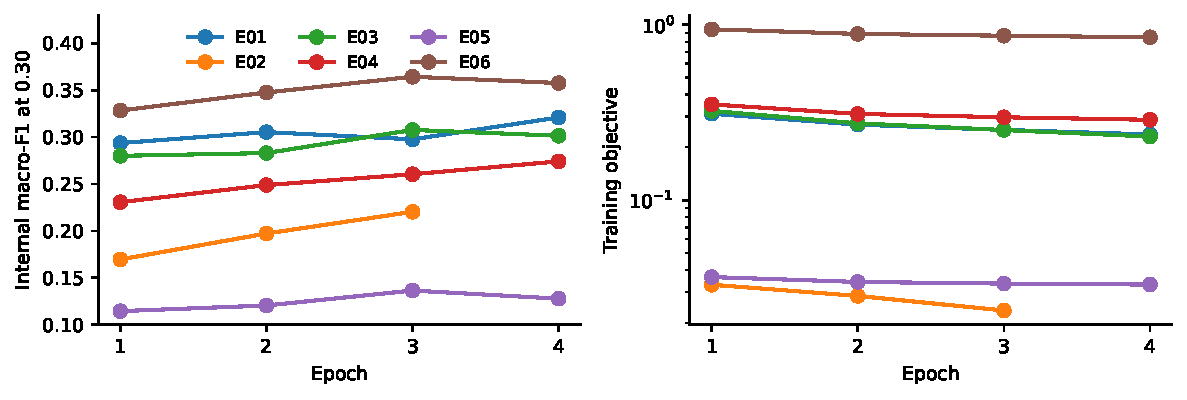
\includegraphics[width=.94\linewidth]{figures/phase5/p5_history.pdf}
\caption{Archived learning curves. Internal validation uses threshold 0.30.
Training objectives differ across runs and their magnitudes are not directly comparable.}
\label{fig:p5-history}
\end{figure}

\subsection{Calibration and submission}
For each checkpoint, development predictions are first evaluated on a
global grid from 0.05 to 0.70 in increments of 0.025. Let \(t_0\) maximize
development macro-F1. For a statute with \(n_j\) positive cases and at
least four positives and four negatives, the same grid selects
\[
 t_j^*=\arg\max_t
 \left[F_{1,j}(t)-0.015\,|t-t_0|\sqrt{6/n_j}\right],
 \qquad
 t_j=\frac{12t_0+n_jt_j^*}{n_j+12}.
\]
Other statutes use \(t_0\). The shrinkage is strongest for labels with
low support. Every calibrated run improves over its global grid optimum
on the calibration data. E02 improves from 0.3741 to 0.3956. Its micro-precision rises from
0.4444 to 0.4590 and micro-recall drops from 0.5656 to 0.5441 on the same
cases. E05 has the
largest improvement (0.0538) and still places sixth. At the internal
threshold of 0.30, E02's best epoch predicted 20.62 labels per case on
average. Its calibrated development mean is 4.64. Both split and
threshold differ, so this comparison illustrates scale rather than a
controlled estimate of calibration's effect on cardinality.

At inference, each threshold is applied to its corresponding sigmoid
probability. If no label clears the threshold, the maximum-probability
label is used. This fallback is specific to test decoding and is absent
from the development metric computation. The submitted archive holds
one root-level \path{prediction.json} with a string \texttt{id} and a
sorted list of unique integer labels under \texttt{pred} for each
test case. There is no maximum label count or ensemble in the six
official submissions.

\begin{figure}[htbp]
\centering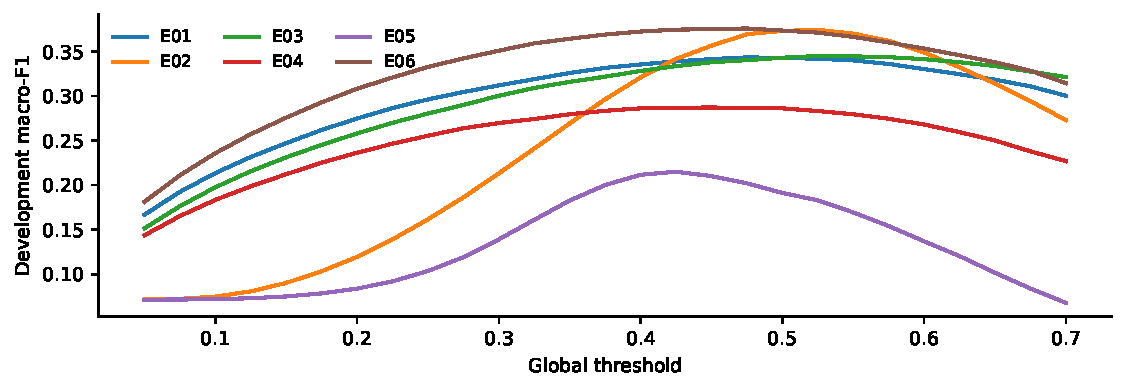
\includegraphics[width=.91\linewidth]{figures/phase5/p5_thresholds.pdf}
\caption{Development global threshold sweep computed from archived logits.}
\label{fig:p5-thresholds}
\end{figure}

\subsection{Experimental progression and official results}
E01 established a parameter-efficient GQA reference. E02 tested whether
the same GQA foundation could benefit from updating the backbone. It
also changed the objective and learning rate, which prevents attribution
of the score difference to full tuning alone. E03 compared selective
decoder unfreezing against full and low-rank GQA adaptation. Its official
score falls between E01 and E02. E04 tested bidirectional windows and
nonlinear adapters, while E05 tested bidirectional encoder states with
attention LoRA. These settings trailed the three causal configurations.
The comparison changes foundation snapshot, trainable weights and, for
E05, loss. E06 tested whether the teacher's multilabel margins could
transfer to a shallower GQA, and it recovered most of E02's official
score with about 55\% as many parameters. Table~\ref{tab:p5-results}
reports the development and official scores for all six runs.

\begin{table}[htbp]
\centering\small
\caption{Local development metrics after per-statute calibration and official
Codabench test macro-F1. All six submissions finished on 28 October 2026.}
\label{tab:p5-results}
\begin{tabular}{lrrrrrr}
\toprule
Run & Global dev F1 & Dev macro-F1 & Dev micro-F1 & Exact set & Official & Submission \\
\midrule
E01 & 0.3432 & 0.3645 & 0.4622 & 0.0294 & 0.3532 & 1014548 \\
E02 & 0.3741 & \textbf{0.3956} & \textbf{0.4979} & \textbf{0.0504} & \textbf{0.3875} & 1014549 \\
E03 & 0.3448 & 0.3689 & 0.4649 & 0.0309 & 0.3565 & 1014550 \\
E04 & 0.2870 & 0.3097 & 0.4000 & 0.0152 & 0.2967 & 1014552 \\
E05 & 0.2150 & 0.2688 & 0.3552 & 0.0043 & 0.2619 & 1014553 \\
E06 & 0.3757 & 0.3954 & 0.4871 & 0.0380 & 0.3842 & 1014554 \\
\bottomrule
\end{tabular}
\end{table}

\begin{figure}[htbp]
\centering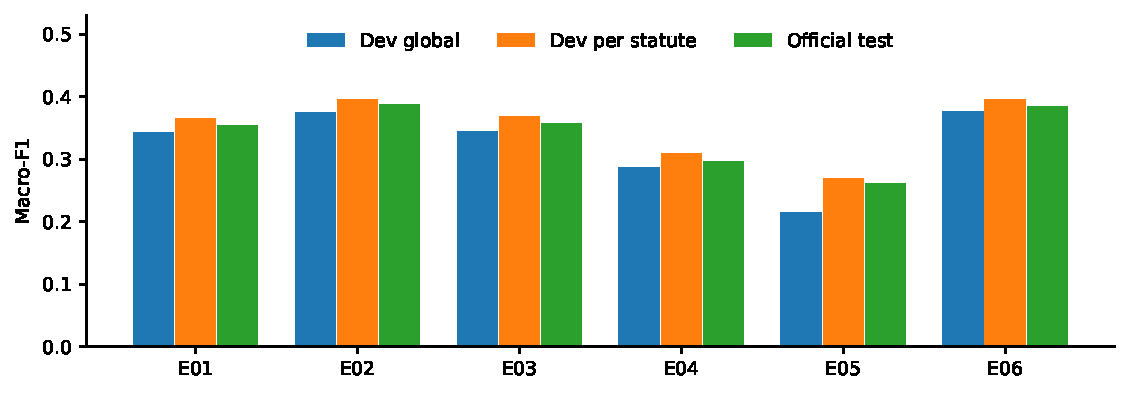
\includegraphics[width=.92\linewidth]{figures/phase5/p5_results.pdf}
\caption{Global and regularized per-statute development results beside official
test macro-F1. The development figures use the threshold-selection set.}
\label{fig:p5-results}
\end{figure}

E02 leads the six project submissions by 0.0033 over E06. Their
calibrated development macro-F1 differs by 0.00025. They predict identical
sets for 1,110 of 13,019 test cases, so their predictions differ on
91.47\% of cases even though their aggregate scores are close. Without
hidden labels, this agreement comparison cannot determine which
disagreements are errors. A single run per configuration and rounded
official scores limit conclusions about the size or stability of the
margin. The E02 winner uses the saved Phase 5 epoch-3 \path{best.pt},
the matching 100 development thresholds and the original Phase 1 BPE.

\subsection{Error analysis}
The E02 development results show both omission and overprediction. For
statute 2 the model detects six of 98 positives and adds 29 false
positives. For statute 8 it detects 12 of 92 positives and adds 217 false
positives. Statute 52 has 228 misses and 372 false positives despite
272 positives. Frequent statute 34 reaches F1 0.8275 and still produces
453 false positives and 444 misses. Support alone does not explain
performance: statutes 20 and 28 have 122 and 151 development positives
and F1 above 0.80. Micro-F1 exceeds macro-F1, while exact-set accuracy
is only 5.04\%, indicating that the model often recovers part of the
statute set. The observed co-occurrences and errors are aggregate
associations. The archive does not identify the evidence span supporting
each label or establish confusion between any specific pair.

\begin{figure}[htbp]
\centering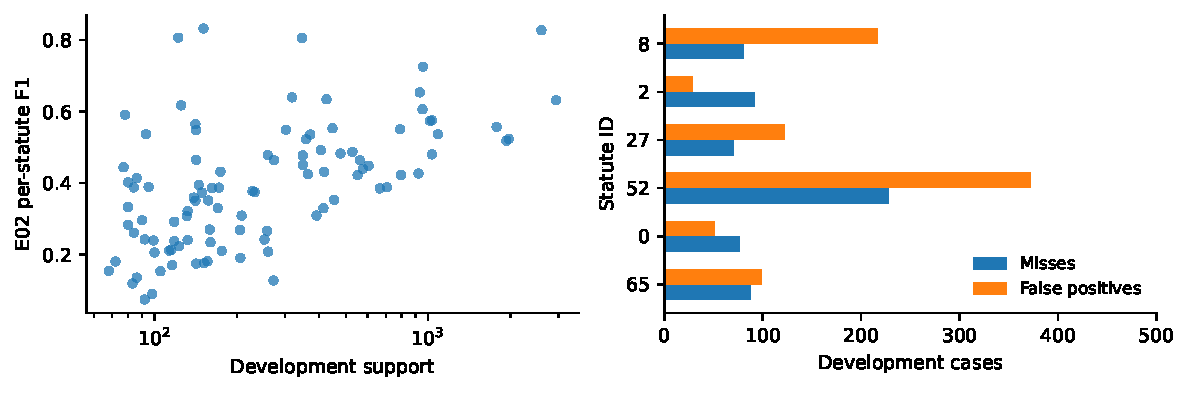
\includegraphics[width=.94\linewidth]{figures/phase5/p5_errors.pdf}
\caption{E02 development performance by statute support and error counts for the six lowest-F1 statutes.}
\label{fig:p5-errors}
\end{figure}

\begin{figure}[htbp]
\centering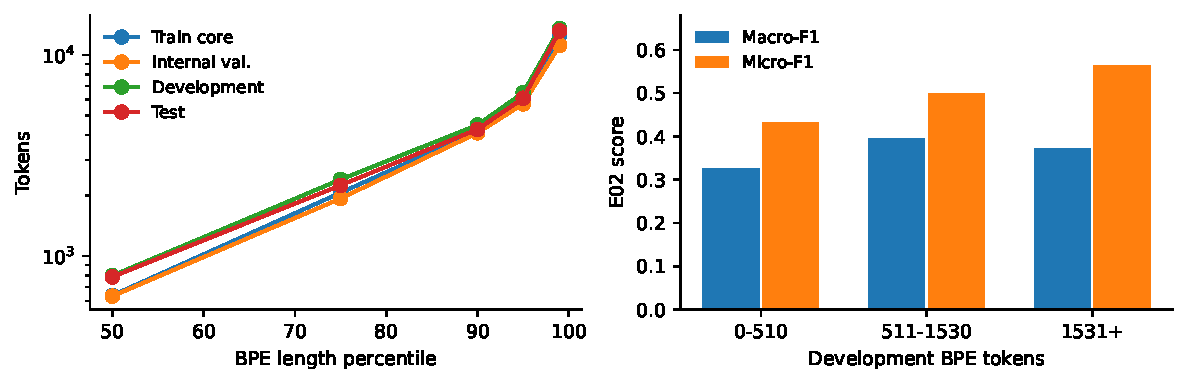
\includegraphics[width=.94\linewidth]{figures/phase5/p5_lengths.pdf}
\caption{BPE length percentiles and E02 development scores by length.
The middle band fits within the aggregate content budget.}
\label{fig:p5-lengths}
\end{figure}

Figure~\ref{fig:p5-lengths} shows development macro-F1 of 0.3266 for
cases up to 510 tokens, 0.3946 for
511--1530 tokens, and 0.3714 beyond 1530. Micro-F1 increases across
the same bins, reaching 0.5634 in the longest group. Class prevalence
and gold cardinality vary by bin. These comparisons do not isolate the
effect of omitted spans, which would require paired predictions with
and without truncation. Similarly, evaluation on a separate calibration
holdout would be needed to quantify the generalization of the fitted
per-statute thresholds.

\subsection{Verification and transition}
The development and test file hashes reproduce the Git LFS pointers at the
pinned dataset revision. All six archived submissions pass ZIP integrity,
statute vocabulary and full test-ID order checks. The release reproduces
all six saved threshold arrays and calibration metrics from development
logits and labels, without exposing the case records. The original E02
checkpoint exceeded the available Drive transfer limit. Synthetic
checkpoint tests and saved-output replay provide distinct checks, while
trained-weight prediction equivalence remains open. Phase 6 uses the
same legal foundation for open-ended abstraction, where evaluation must
compare generated text rather than a fixed inventory of statutes.
